% Layer-SAM, left to right, at slide size (the poster's plots/nfo/architecture.tex runs top to bottom).
% Colours as in the SAM2 paper figure: green encoder, orange decoder, lavender prompt encoder, pink memory (not used);
% blue outline = trained by us. Needs \Fire / \Ice (defined by plots/nfo/architecture.tex) and ColOurs / ColSamurai.
\definecolor{SamEnc}{HTML}{D4F5C4}\definecolor{SamEncD}{HTML}{8FCF79}
\definecolor{SamDec}{HTML}{FDE6C8}\definecolor{SamDecD}{HTML}{E9B676}
\definecolor{SamPrm}{HTML}{DEDDFB}\definecolor{SamPrmD}{HTML}{9E9BE6}
\definecolor{SamMem}{HTML}{F9DDF0}\definecolor{SamMemD}{HTML}{E7A9D3}
\begin{tikzpicture}[x=1cm, y=1cm, font=\PraesentationSchriftgroesseKlein\selectfont,
    a/.style={-{Latex[length=2.2mm]}, line width=0.9pt, draw=black!75},
    blk/.style={rounded corners=3pt, line width=0.9pt, align=center, inner sep=3pt},
    feat/.style={draw=SamEncD, fill=SamEnc!70, line width=0.7pt, minimum size=6.5mm, inner sep=0pt}]
  % inputs
  \foreach \n/\y/\f/\l in {X/2.5/inputs_0/{frame $t$\\{\color{black!60}tracker box}},
                           C/0/inputs_2/{integral image\\{\color{black!60}6 past frames}},
                           B/-2.5/inputs_1/{empty scene\\{\color{black!60}once per scene}}} {
    \node[inner sep=0pt] (\n) at (0, \y) {\includegraphics[height=2.1cm]{plots/nfo/\f.jpg}};
    \node[anchor=east, align=right] at (-1.0, \y) {\l};
  }
  % shared, frozen image encoder
  \node[blk, draw=SamEncD, fill=SamEnc, minimum width=1.1cm, minimum height=7.3cm] (enc) at (2.2, 0)
        {\rotatebox{90}{\Ice\ \textbf{image encoder}\ \ {\color{black!60}same weights for all three}}};
  \foreach \n/\y/\s in {X/2.5/t, C/0/C, B/-2.5/B} {
    \draw[a] (\n.east) -- (1.65, \y);
    \node[feat] (f\n) at (3.8, \y) {$F_{\s}$};
    \draw[a] (2.75, \y) -- (f\n.west);
  }
  % adapter
  \node[blk, draw=ColOurs, fill=ColOurs!12, line width=1.4pt, minimum width=2.5cm, minimum height=4.2cm] (ad) at (6.3, -1.25)
        {\Fire\ \textbf{adapter}\\0.7\,M\\[2mm]{\color{black!60}strides}\\{\color{black!60}16 $\to$ 8 $\to$ 4}};
  \draw[a] (fC.east) -- (fC.east -| ad.west);
  \draw[a] (fB.east) -- (fB.east -| ad.west);
  \draw[a] (5.5, 2.5) -- (5.5, 0.85);
  % corrected frame features
  \node[circle, draw=black!80, line width=1pt, minimum size=5.5mm, inner sep=0pt] (plus) at (8.6, 2.5) {$+$};
  \draw[a] (fX.east) -- (plus.west);
  \draw[a] (ad.east) -| node[pos=0.75, right] {$R$} (plus.south);
  % decoder, prompt encoder, tracker
  \node[blk, draw=SamDecD, fill=SamDec, minimum width=2.9cm, minimum height=9mm] (dec) at (11.2, 2.5) {\Ice\ \textbf{mask decoder}};
  \draw[a] (plus.east) -- node[above] {$\hat F_t$} (dec.west);
  \node[blk, draw=SamPrmD, fill=SamPrm, minimum width=2.9cm, minimum height=9mm] (pe) at (11.2, 0.3) {\Ice\ \textbf{prompt encoder}};
  \draw[a] (pe.north) -- (dec.south);
  \node[blk, draw=black!70, fill=white, line width=1.0pt, minimum width=2.9cm, minimum height=9mm] (trk) at (11.2, -2.0)
        {\textbf{tracker}\\{\color{black!60}box + point}};
  \draw[a] (trk.north) -- (pe.south);
  \draw[a, draw=black!45] (fB.south) -- (3.8, -3.75) -| node[pos=0.25, below, text=black!60] {change of $F_t$ against $F_B$} (trk.south);
  % output, memory not used, legend
  \node[inner sep=0pt] (M) at (14.4, 2.5) {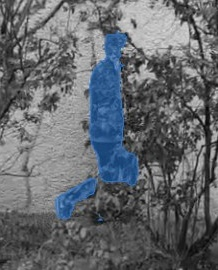
\includegraphics[height=2.1cm]{plots/nfo/inputs_6.jpg}};
  \draw[a] (dec.east) -- (M.west);
  \node[above=0.5mm of M] {mask};
  \node[blk, draw=SamMemD, fill=SamMem!50, dashed, text=black!55, minimum width=2.6cm] (mem) at (14.4, -0.4)
        {memory of\\past masks\\not used};
  \draw[a, draw=black!35, dashed] (M.south) -- node[text=ColSamurai, font=\large\bfseries, fill=white, inner sep=0pt] {$\times$} (mem.north);
  \node[align=left, anchor=north] at (14.4, -1.8) {\Fire\ trained\\\Ice\ frozen SAM2.1};
\end{tikzpicture}
